\PassOptionsToPackage{quiet}{fontspec}
\documentclass[12pt,a4paper]{article}
\usepackage{thesis} % 格式控制
\usepackage{indentfirst}
\usepackage{enumitem}
\usepackage{amsmath} % 数学公式支持
\usepackage{amsfonts} % 数学字体支持
\usepackage{amssymb} % 数学符号支持
\usepackage{graphicx} % 图片插入支持
\usepackage{float} % 浮动体位置控制，支持 [H] 选项
\usepackage{caption} % 图表标题格式控制
\usepackage{geometry} % 页面布局控制
\usepackage{setspace} % 行距控制
\usepackage{xeCJK} % 中文字体支持
\usepackage{fontspec} % 字体设置
\usepackage[most]{tcolorbox} % 高亮按键命令
\usepackage{listings} % 代码高亮
\usepackage[table]{xcolor} % 颜色支持
\setlength{\parindent}{2em} % 控制首行缩进  
\addtolength{\parskip}{3pt} % 控制段落距离  
\onehalfspacing % 1.5倍行距  
\graphicspath{{./figures/}} % 指定图片所在文件夹  
\setCJKmainfont{SimSun}

% 配置lstlisting样式
\lstset{
    basicstyle=\ttfamily\small,
    breaklines=true,
    frame=single,
    numbers=left,
    numberstyle=\tiny\color{gray},
    backgroundcolor=\color{gray!10},
    keywordstyle=\color{blue},
    commentstyle=\color{green!60!black},
    stringstyle=\color{red},
    showstringspaces=false,
    tabsize=4,
    captionpos=b,
    xleftmargin=2em,
    xrightmargin=2em,
    aboveskip=1em,
    belowskip=1em
}

\classname{\heiti\bfseries 信息电子学物理基础}  % 设置课程名称
\makepagestyle{}{}

\newtcbox{\keyblue}{on line,
  colframe=blue!60!black, colback=blue!5,
  boxrule=0.8pt, arc=2pt, boxsep=0pt, left=3pt, right=3pt, top=2pt, bottom=2pt,
  tcbox raise base, fontupper=\ttfamily\small}

\newtcbox{\pathbox}{on line,
  colframe=green!60!black, colback=green!5,
  boxrule=0.8pt, arc=2pt, boxsep=0pt, left=3pt, right=3pt, top=2pt, bottom=2pt,
  tcbox raise base, fontupper=\ttfamily\small}

\begin{document}
\maketitlepage{“流光守护”智能夜跑服设计}{玉泉教7-104}{}{}{\today}{林时胜} %封面页 

\maketoc

\section{设计背景与核心需求}

\subsection{设计背景与现状分析}

\subsubsection{设计背景}
随着"全民健身"战略的推进,夜跑已成为现代都市人群释放压力、保持健康的重要生活方式。然而,夜间光线昏暗、交通环境复杂,导致夜跑安全事故频发。传统的安全防护装备主要依赖被动反光材料(如3M反光条),只有在被强光(如车灯)直接照射时才有效,存在明显的"视觉盲区"。

与此同时,柔性电子技术取得了突破性进展。特别是\textbf{本征可拉伸(Intrinsically Stretchable)}的量子点发光二极管(QLED)技术,不仅具备高色彩饱和度和高亮度,还能在发生形变(拉伸、弯曲)时保持性能稳定,这使其成为下一代智能穿戴设备最理想的光源\cite{kim2024intrinsically}。

\subsubsection{现有解决方案的不足}
目前的夜跑装备和发光服饰市场存在以下主要痛点:

\begin{itemize}
    \item \textbf{被动防护局限性:} 传统反光衣在无光源照射(如黑暗公园角落)时完全失效,无法主动警示。
    
    \item \textbf{舒适度差:} 现有的主动发光衣多采用硬质LED灯带或EL冷光线,质地僵硬、透气性差,且难以适应人体关节的大幅度运动。
    
    \item \textbf{热管理与防水难题:} 传统柔性发光器件在出汗或雨天环境下容易失效,且在大电流驱动下的自热问题会降低器件寿命。据GW Baek et al. (2023)研究\cite{choi2023highly}。
\end{itemize}

\subsubsection{需求分析与应用场景}
基于上述背景,"流光守护"智能夜跑服的设计需求主要集中在以下几点:

\begin{enumerate}
    \item \textbf{主动安全性:} 实现高亮度的自主发光(>1000 cd/m²),确保360度可视。
    
    \item \textbf{柔性与耐用性:} 必须使用具备防水、耐汗液腐蚀且散热良好的柔性封装技术。
    
    \item \textbf{智能交互:} 光色或闪烁频率应能随跑者的运动状态(心率、速度)动态变化。
\end{enumerate}

目标应用场景:城市夜跑、夜间马拉松赛事、光线不足的户外徒步以及骑行安全警示。

\subsection{核心功能设计}
为了打造"流光守护"这一概念,本系统将集成以下三大核心功能:

\textbf{全柔性主动发光警示(Active Flexible Illumination):} 利用顶发射(Top-emitting)结构的柔性QLED器件,集成在超薄柔性衬底(如PEN或PET)上。这种结构能显著提高光的出射效率,解决传统发光服饰亮度不足的问题,同时配合金属箔衬底解决散热问题。H Yu et al. (2022)的研究证实了这一技术路径\cite{chen2022high}。

\textbf{运动节律同步(Bio-Rhythm Synchronization):} 内置微型运动传感器(IMU),采集跑者的步频信号。通过微控制器(MCU)算法,控制QLED的发光频率与步频"呼吸"同频,在视觉上强化运动节奏感。

\textbf{生理状态可视化反馈:} 设定安全阈值,当跑者心率过高或运动负荷过大时,衣物发光颜色由冷色调(如蓝色)自动渐变为警示色(如红色),直观地提醒用户调整强度。

\begin{figure}[H]
\centering
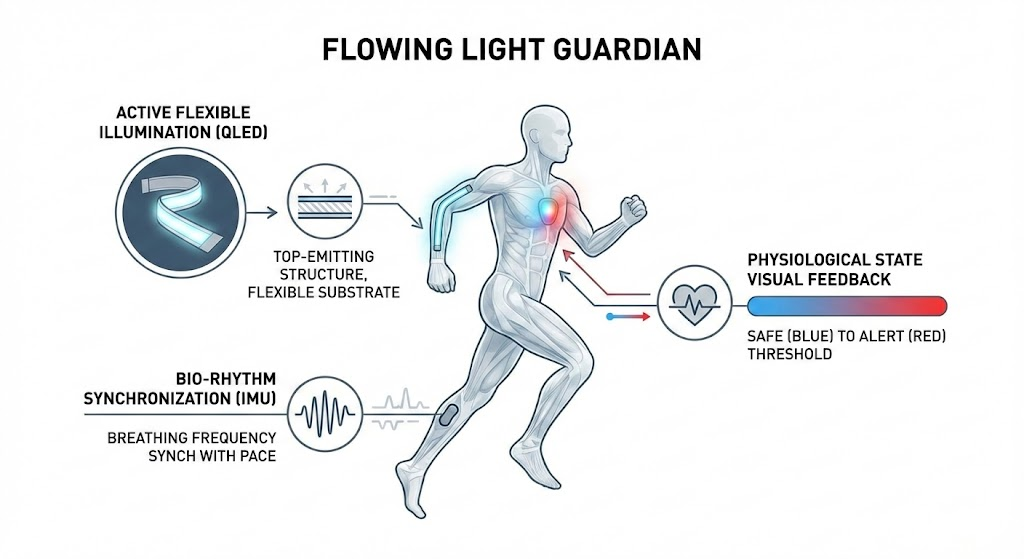
\includegraphics[width=0.8\textwidth]{p1.jpg}
\caption{核心功能设计示意图}
\label{fig:core_functions}
\end{figure}

\subsection{工作环境与器件要求}
为了实现上述功能,并确保设备在复杂的运动环境下长期稳定工作,对QLED器件及其封装提出了严格的物理与光学要求。

\subsubsection{机械与环境耐受性要求}

\begin{itemize}
    \item \textbf{可拉伸性(Stretchability):} 考虑到人体关节运动,器件需能承受至少50\%的拉伸应变而不发生断裂或明显亮度衰减\cite{kim2024intrinsically}。
    
    \item \textbf{防水抗汗(Waterproof \& Sweat-proof):} 必须采用高致密的薄膜封装(如Parylene C/SU-8双层封装),以抵御汗液中的盐分和水分侵蚀,确保在潮湿环境下正常工作。GW Baek et al. (2023)的研究提供了封装技术支持\cite{choi2023highly}。
\end{itemize}

\begin{figure}[H]
\centering
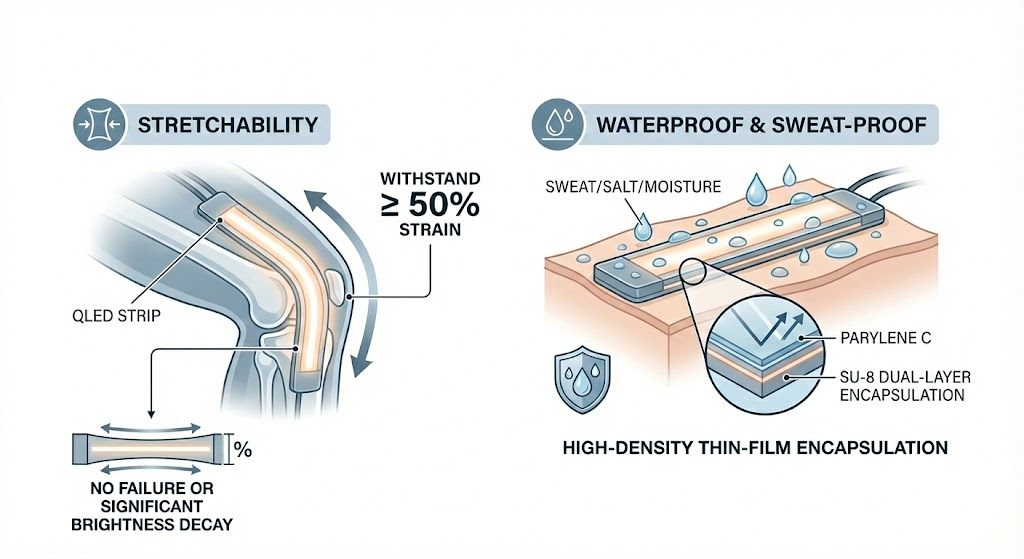
\includegraphics[width=0.8\textwidth]{p2.jpg}
\caption{机械与环境耐受性要求示意图}
\label{fig:mechanical_requirements}
\end{figure}

\subsubsection{发光性能要求}

\begin{itemize}
    \item \textbf{高亮度(High Luminance):} 为对抗城市环境光干扰,器件在工作电压下的峰值亮度需达到\textbf{5,000 cd/m\textsuperscript{2}}(相当于高端智能手机屏幕亮度),日常警示模式下维持在1,000-2,000 cd/m\textsuperscript{2}。驱动电压需$<6$V以匹配便携锂电池。H Yu et al. (2022)已实现类似性能指标\cite{chen2022high}。
    
    \item \textbf{热管理策略:} 考虑到莱卡织物的低导热特性($\lambda \approx 0.1$ W/m·K),必须采用\textbf{脉冲驱动模式(Pulsed Operation)}而非连续发光,占空比控制在$<30\%$。同时利用Ag NWs阳极的横向散热通道,配合透气织物的自然对流,将器件稳态温升限制在$\Delta T < 15^{\circ}$C以内,避免热猝灭\cite{kim2024intrinsically}。
\end{itemize}

\begin{figure}[H]
\centering
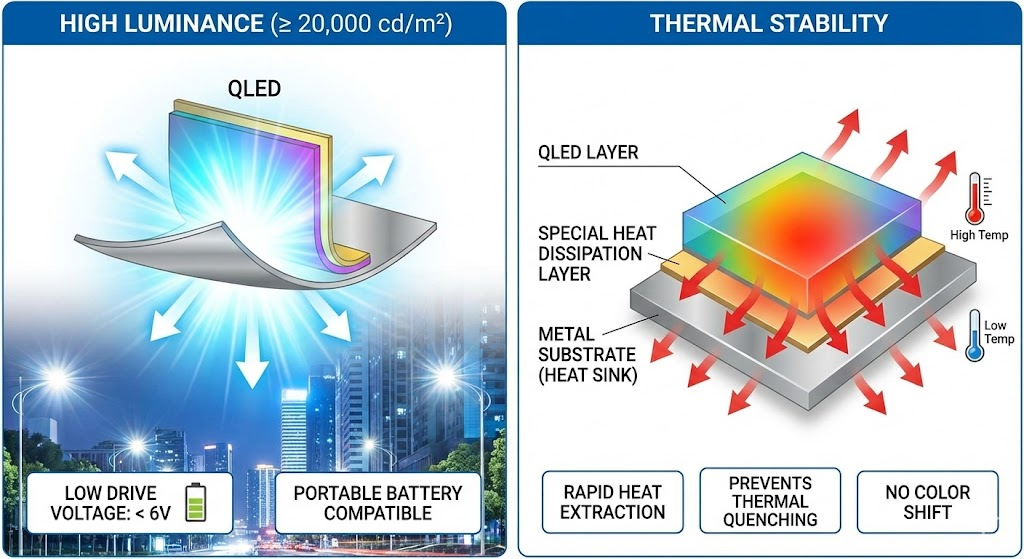
\includegraphics[width=0.8\textwidth]{p3.jpg}
\caption{发光性能要求示意图}
\label{fig:luminance_requirements}
\end{figure}

\clearpage
\section{QLED设计指标与要求}

\subsection{QLED工作环境与寿命指标}
为了适应夜跑、马拉松及户外徒步等复杂场景,QLED器件必须满足以下严苛的环境耐受性指标:

\subsubsection{工作温度范围(Operating Temperature)}

\textbf{指标设定:} $-10^{\circ}\text{C} \sim 85^{\circ}\text{C}$

\textbf{设计依据:} 依据S Mokarian Zanjani et al. (2023)的热循环实验数据,高性能红/绿/蓝QLED在此温度区间内能保持较高的量子效率(EQE),且未出现灾难性故障\cite{haghighi2023investigation}。$-10^{\circ}\text{C}$覆盖冬季户外环境,$85^{\circ}\text{C}$覆盖夏季体温叠加器件大电流驱动时的自热结温。

\textbf{热猝灭阈值:} 设计散热结构时,需确保核心发光层(EML)温度不超过$90^{\circ}\text{C}$,防止量子点配体脱落导致不可逆的光衰。

\subsubsection{环境与寿命指标(Environment \& Lifetime)}

\begin{itemize}
    \item \textbf{使用寿命($T_{50}$):} 在初始亮度$L_0 = 5000 \text{ cd/m}^2$的高亮模式下,连续工作寿命需达到5,000小时以上。
    
    \item \textbf{防水抗湿(Humidity Resistance):} 必须达到IP67级防水。由于柔性器件对水氧极度敏感,必须采用多层薄膜封装(TFE),要求水汽透过率(WVTR) $< 10^{-5} \text{ g m}^{-2} \text{ day}^{-1}$\cite{lee2023truly}。
    
    \item \textbf{机械寿命:} 能够承受10,000次半径$R=3\text{mm}$的反复弯曲,亮度衰减$< 10\%$。
\end{itemize}

\subsection{发光频率/波长}

本设计采用\textbf{RGB三基色电致发光}方案,精准对应人眼视觉敏感区:

\begin{itemize}
    \item \textbf{警示红(Alert Red):} $\lambda_{peak} = 625 \text{ nm}$(频率$\sim 480 \text{ THz}$),用于心率预警。
    
    \item \textbf{安全绿(Safety Green):} $\lambda_{peak} = 525 \text{ nm}$(频率$\sim 571 \text{ THz}$),用于常亮照明。
    
    \item \textbf{深邃蓝(Cool Blue):} $\lambda_{peak} = 460 \text{ nm}$(频率$\sim 652 \text{ THz}$),用于配速呼吸灯效。
    
    \item \textbf{色纯度:} 半峰全宽(FWHM) $< 25 \text{ nm}$,确保色彩穿透力强。
\end{itemize}


\clearpage
\section{QLED器件结构与材料选择}

\subsection{QLED器件的常用器件结构}

QD-LED器件的结构设计是实现其高性能发光特性的关键。一个典型的QD-LED器件结构包括以下几个主要部分:

\begin{figure}[H]
\centering
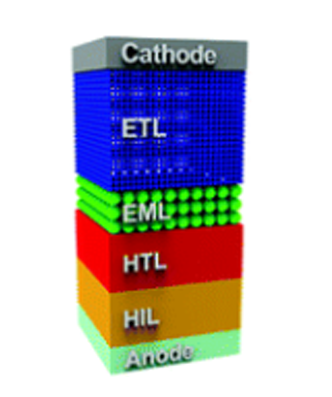
\includegraphics[width=0.3\textwidth]{p5.png}
\caption{QD-LED器件结构示意图\cite{bang2021technology}}
\label{fig:qled_structure}
\end{figure}

\begin{table}[H]
\centering
\caption{QD-LED器件各功能层说明}
\small
\begin{tabular}{ll}
\hline
\hline
\textbf{功能层} & \textbf{功能描述} \\
\hline
\begin{tabular}[c]{@{}l@{}}基底\\(Substrate)\end{tabular} & \begin{tabular}[c]{@{}l@{}}通常由玻璃或塑料构成,用于支撑整个器件结构\end{tabular} \\
\hline
\begin{tabular}[c]{@{}l@{}}阳极\\(Anode)\end{tabular} & \begin{tabular}[c]{@{}l@{}}通常由透明的导电材料构成,如ITO(铟锡氧化物),\\其作用是允许光线透过并作为电流的注入端\end{tabular} \\
\hline
\begin{tabular}[c]{@{}l@{}}空穴注入层\\(HIL)\end{tabular} & \begin{tabular}[c]{@{}l@{}}位于阳极之上,其功能是促进空穴从阳极注入到量子点发光层。\\这一层通常由有机小分子或聚合物构成,具有良好的空穴传输性能\end{tabular} \\
\hline
\begin{tabular}[c]{@{}l@{}}空穴传输层\\(HTL)\end{tabular} & \begin{tabular}[c]{@{}l@{}}紧邻空穴注入层,负责将空穴从空穴注入层传输到量子点发光层\end{tabular} \\
\hline
\begin{tabular}[c]{@{}l@{}}量子点发光层\\(QD Layer)\end{tabular} & \begin{tabular}[c]{@{}l@{}}这是QD-LED器件的核心部分,由量子点材料构成。\\量子点的尺寸和组成决定了发射光的颜色。这一层的设计需要\\精确控制量子点的尺寸和分布,以实现最佳发光效率和颜色稳定性\end{tabular} \\
\hline
\begin{tabular}[c]{@{}l@{}}电子传输层\\(ETL)\end{tabular} & \begin{tabular}[c]{@{}l@{}}位于量子点发光层之上,其作用是促进电子从阴极注入到\\量子点发光层,并阻止空穴的过度注入,从而提高器件的\\发光效率和寿命\end{tabular} \\
\hline
\begin{tabular}[c]{@{}l@{}}阴极\\(Cathode)\end{tabular} & \begin{tabular}[c]{@{}l@{}}通常由低功函数的金属构成,如钙、铝或其合金,用于电子的注入\end{tabular} \\
\hline
\hline
\end{tabular}
\end{table}

\subsection{材料与参数设计}

据Kim et al. (2024)在Nature Electronics发表的"本征可拉伸QLED"技术路线,确定本设计的最终材料\cite{kim2024intrinsically}。与传统刚性器件不同,本设计采用了\textbf{正置结构(Conventional Structure)},即阳极在下、阴极在上。该结构利用层级化的空穴注入层,配合顶部液态金属阴极,完美解决了器件在50\%拉伸应变下的电荷传输与机械稳定性问题。

\subsubsection{本征可拉伸器件结构(Device Structure)}

下图展示了"流光守护"夜跑服发光单元的完整层叠结构。该结构由上下两层紫外固化聚氨酯(PUA)封装,形成类似"三明治"的防水保护结构。

\begin{figure}[H]
\centering
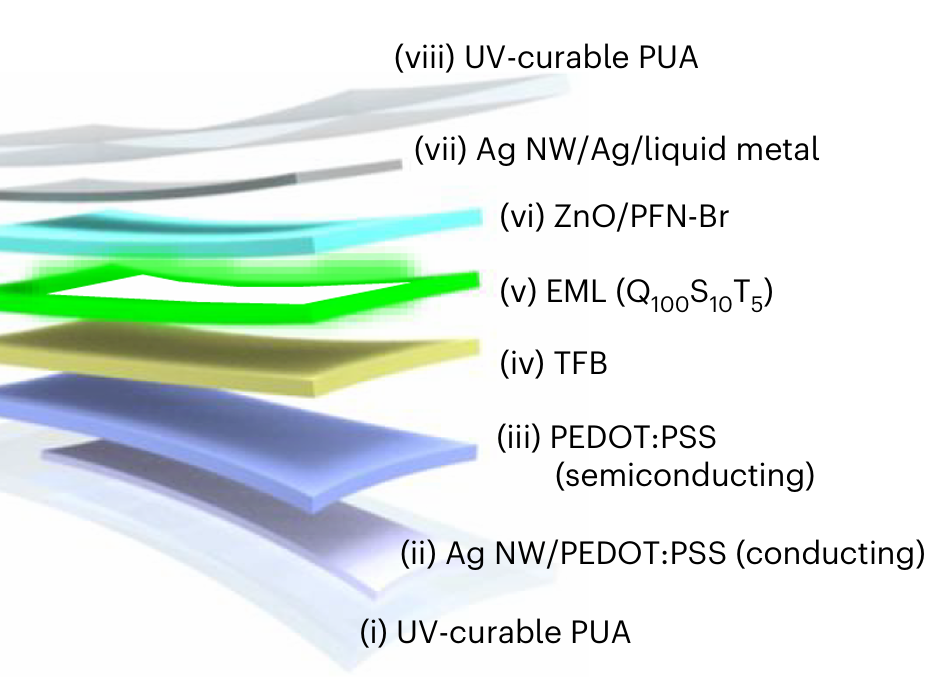
\includegraphics[width=0.7\textwidth]{p4.png}
\caption{本征可拉伸QLED的全柔性器件层叠结构示意图(源自Kim et al., 2024)。该结构采用了正置堆叠,利用三元混合发光层(EML)和液态金属复合阴极实现高拉伸性\cite{kim2024intrinsically}}
\label{fig:stretchable_structure}
\end{figure}


\subsubsection{详细材料参数表}

为了实现Section 2.1设定的IP67防水与高拉伸寿命指标,各功能层的选材与参数设计如下表所示:

\begin{table}[H]
\centering
\caption{QLED器件各功能层材料及其关键参数}
\small
\begin{tabular}{llll}
\hline
\hline
\textbf{层级} & \textbf{材料选择} & \textbf{关键参数} & \textbf{设计理由} \\
\hline
\begin{tabular}[c]{@{}l@{}}封装/基底\end{tabular} & \begin{tabular}[c]{@{}l@{}}UV-curable PUA\\(聚氨酯丙烯酸酯)\end{tabular} & \begin{tabular}[c]{@{}l@{}}杨氏模量$E \approx 10$ MPa\\透光率$> 90\%$\end{tabular} & \begin{tabular}[c]{@{}l@{}}如图中层(i)和(viii)所示,PUA\\提供极佳的皮肤贴合性与防水\\保护,像皮肤一样随肢体拉伸\end{tabular} \\
\hline
\begin{tabular}[c]{@{}l@{}}复合阳极\end{tabular} & Ag NWs / PEDOT:PSS & 方块电阻$R_{sq} < 15\,\Omega/\square$ & \begin{tabular}[c]{@{}l@{}}银纳米线网络提供高导电性,\\PEDOT:PSS填充空隙并平滑表面\\粗糙度,防止漏电流\end{tabular} \\
\hline
\begin{tabular}[c]{@{}l@{}}空穴传输层\end{tabular} & TFB & HOMO $\approx 5.4$ eV & \begin{tabular}[c]{@{}l@{}}纯聚合物层,用于阶梯式能级\\匹配,将空穴有效传输至发光层\\内部的TFB岛状区域\end{tabular} \\
\hline
\begin{tabular}[c]{@{}l@{}}核心发光层\\(EML)\end{tabular} & \begin{tabular}[c]{@{}l@{}}三元纳米复合材料\\($Q_{100}S_{10}T_5$)\end{tabular} & \begin{tabular}[c]{@{}l@{}}配方: QDs (100) : \\SEBS (10) : TFB (5)\\结构: 相分离纳米岛状结构\end{tabular} & \begin{tabular}[c]{@{}l@{}}\textbf{核心技术:} 量子点提供高色纯度\\发光;SEBS弹性体基质承担机械\\拉伸应力;TFB形成互穿网络\\传输电荷\end{tabular} \\
\hline
\begin{tabular}[c]{@{}l@{}}电子传输层\end{tabular} & ZnO NPs / PFN-Br & \begin{tabular}[c]{@{}l@{}}电子迁移率\\$\mu_e \sim 10^{-3}$ cm$^2$/Vs\end{tabular} & \begin{tabular}[c]{@{}l@{}}经典的无机电子传输材料,\\PFN-Br修饰层可降低界面偶极\\势垒,增强电子注入效率\end{tabular} \\
\hline
\begin{tabular}[c]{@{}l@{}}复合阴极\end{tabular} & \begin{tabular}[c]{@{}l@{}}EGaIn / Ag NWs\\(液态金属/银)\end{tabular} & 临界拉伸应变$\varepsilon > 100\%$ & \begin{tabular}[c]{@{}l@{}}\textbf{关键设计:} 由于是正置结构,\\顶层阴极必须承受最大形变。\\液态金属(EGaIn)确保电极在\\拉伸时不发生断裂\end{tabular} \\
\hline
\hline
\end{tabular}
\end{table}

\clearpage
\section{QLED器件的精密制备工艺}

本研究采用全溶液加工与喷涂沉积相结合的工艺,在弹性体基底上构建本征可拉伸QLED器件。核心工艺流程涵盖\textbf{复合阳极转印、功能层逐层旋涂、复合阴极沉积及系统封装}四大步骤。

\subsection{复合阳极转印}

为解决传统ITO电极易脆裂的问题,采用嵌入式Ag NWs/PEDOT:PSS复合阳极结构\cite{choi2023highly}。

\begin{enumerate}
    \item \textbf{牺牲层处理:} 对硅晶圆表面进行ODTS自组装单分子层处理,降低表面能以利于后续剥离。
    
    \item \textbf{Ag NW网络构建:} 通过荫罩将Ag NWs溶液(0.1 wt\% 异丙醇分散液)喷涂于硅片上,形成导电网络。
    
    \item \textbf{PUA弹性体转印:} 将PUA树脂浇筑在Ag NW网络上,经紫外光固化后揭下,使Ag NWs半嵌入PUA基底表面,形成平整且高导电的电极层。
    
    \item \textbf{PEDOT:PSS修饰:} 喷涂掺杂5 wt\% DMSO和1 wt\% FS-31的高导电PEDOT:PSS(PH1000)。DMSO破坏PEDOT与PSS的静电相互作用,诱导PEDOT形成线性富集域,显著提升电极拉伸性与导电性\cite{kim2024intrinsically}。
\end{enumerate}

\subsection{功能层逐层旋涂}

在转印完成的阳极之上,依次制备空穴功能层、发光层和电子传输层\cite{kim2024intrinsically}。

\begin{enumerate}
    \item \textbf{空穴注入层(HIL):} 旋涂掺杂1 wt\% FS-31的半导体型PEDOT:PSS(AI 4083),形成厚度约30 nm的薄膜。FS-31有效抑制拉伸过程中的裂纹扩展,在60\%应变下保持结构完整。
    
    \item \textbf{空穴传输层(HTL):} 在手套箱环境中旋涂TFB溶液,成膜厚度约20 nm。
    
    \item \textbf{三元发光层(EML):} 将CdSe/ZnS量子点、SEBS-g-MA弹性体与TFB聚合物按$Q_{100}S_{10}T_{5}$比例混合溶于氯苯,一步旋涂(厚度35 nm)。利用溶剂挥发时各组分表面能差异($\gamma_{\text{TFB}} < \gamma_{\text{QD}} < \gamma_{\text{SEBS}}$),实现自发垂直相分离:TFB在底部富集辅助空穴注入,量子点分散于弹性体基质中保证拉伸稳定性。
    
    \item \textbf{电子传输层(ETL):} 旋涂ZnO纳米颗粒与PFN-Br的乙醇混合溶液(2.5 mg/mL),形成40 nm厚的ETL。乙醇溶剂的正交性避免破坏下层EML,PFN-Br提高ZnO层断裂韧性,拉伸时仅呈现微裂纹而非贯穿性断裂。
\end{enumerate}

\subsection{复合阴极沉积}

顶电极采用多层复合结构以克服金属薄膜在拉伸时的断路问题\cite{kim2024intrinsically, ma2021permeable}。

\begin{enumerate}
    \item \textbf{Ag NWs骨架层:} 在ETL表面喷涂Ag NWs网格,建立基础导电骨架。
    
    \item \textbf{界面改性层:} 沉积超薄Ag膜,改善后续液态金属的润湿性与附着力。
    
    \item \textbf{液态金属修复层:} 喷涂EGaIn液态金属层。液态金属填充Ag NWs网格空隙,构建具有"自修复"能力的逾渗网络,确保器件在50\%以上拉伸应变下维持稳定的电子注入通道。
\end{enumerate}


\begin{figure}[H]
\centering
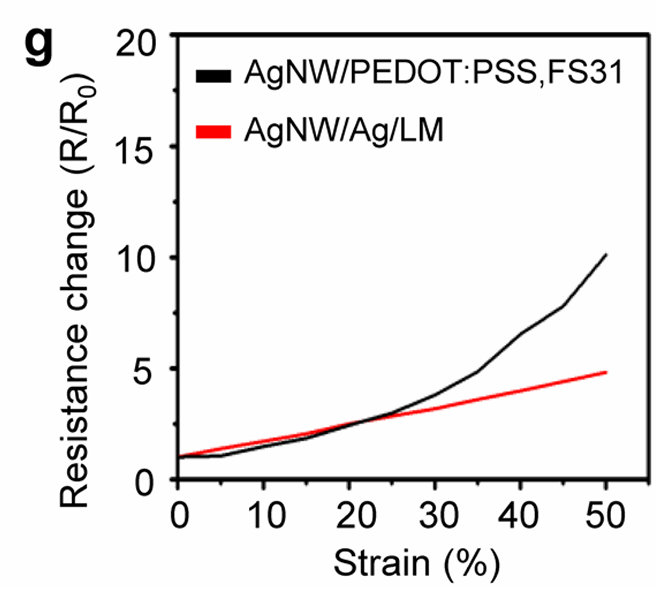
\includegraphics[width=0.5\textwidth]{p11.png}
\caption{阳极与阴极在拉伸过程中的电阻变化对比\cite{kim2024intrinsically}。红线(AgNW/Ag/LM)代表液态金属复合阴极,黑线(AgNW/PEDOT:PSS)代表传统阳极。液态金属复合阴极在50\%拉伸应变下电阻相对保持恒定($R/R_0 \approx 1$),充分证明了"自修复"逾渗网络的优越性。}
\label{fig:electrode_strain_resistance}
\end{figure}

\subsection{系统封装}

最后,在器件顶部旋涂并紫外固化一层PUA树脂,形成致密保护层,隔绝水氧并防止液态金属泄漏\cite{kim2024intrinsically}。

\clearpage
\section{织物集成与加工工艺设计}

\subsection{织物基底选型与界面平坦化}

\subsubsection{织物基底选型}

针对夜跑服高动态、多汗液的应用环境,基底材料需在机械性能上与QLED器件(断裂伸长率$>500\%$)实现模量匹配。

\textbf{选材方案:} 选用Lycra\textsuperscript{\textregistered}(莱卡)经编织物(80\%聚酯纤维+20\%氨纶)。

\textbf{设计依据:} 相比于梭织面料,经编莱卡具有各向同性的高弹性($\sim$300\%应变),能最大限度减少人体关节活动时对贴附器件的剪切应力。

\subsubsection{紫外固化树脂平坦化工艺(UV-Resin Planarization)}

\textbf{技术痛点:} 传统纺织品的表面粗糙度(RMS)通常在$20 \sim 50\,\mu$m级别,而QLED的核心功能层厚度仅为$100 \sim 200$ nm,直接在织物上制备器件会导致严重的漏电流甚至短路。

\textbf{工艺实现:} 采用"全织物QLED"平坦化方案:

\begin{enumerate}
    \item \textbf{旋涂:} 将生物相容性的紫外固化聚氨酯丙烯酸酯(PUA)树脂涂布于莱卡面料选定区域。
    
    \item \textbf{相变控制:} 利用PUA树脂的粘度特性,使其部分渗透进纤维束内部(形成机械互锁锚点),同时在表面形成连续薄膜。
    
    \item \textbf{固化:} 经365nm UV光照固化后,织物表面的RMS粗糙度可降低至$< 10$ nm,构建出类似玻璃般平整但仍具柔性的微纳加工界面。
\end{enumerate}

\subsection{异质转印集成技术}

为了规避传统光刻工艺中显影液对织物纤维的腐蚀,本设计采用\textbf{"热释放辅助的逆向转印技术(Thermal-Release Assisted Reverse Transfer)"}。该方法已被证明可实现接近100\%的转移良率\cite{kim2024recent}。

\subsubsection{转印原理与工艺流程}

此步骤的目的是将第4节制备好的精密器件,从玻璃基底完整地"复制"到粗糙的织物上。由于器件已预先制备完成,织物本身完全免受化学溶剂和高温退火的侵蚀。

\textbf{热压键合与释放(Hot-Press Bonding \& Release):}

\begin{itemize}
    \item \textbf{界面粘合剂:} 在平坦化的莱卡织物表面预涂一层50$\,\mu$m厚的TPU(热塑性聚氨酯)热熔胶膜。
    
    \item \textbf{转印过程:} 将玻璃载体倒扣于织物上,施加5 bar压力并加热至$130^{\circ}$C。
    
    \item \textbf{双重相变机制:} 在此温度下,织物侧的TPU熔融产生强粘附力(锚定器件),而玻璃侧的TRT胶带失去粘性(释放器件)。
    
    \item \textbf{完成转移:} 冷却后揭去玻璃,QLED器件即被无损地"复制"到了织物表面。
\end{itemize}

\begin{figure}[H]
\centering
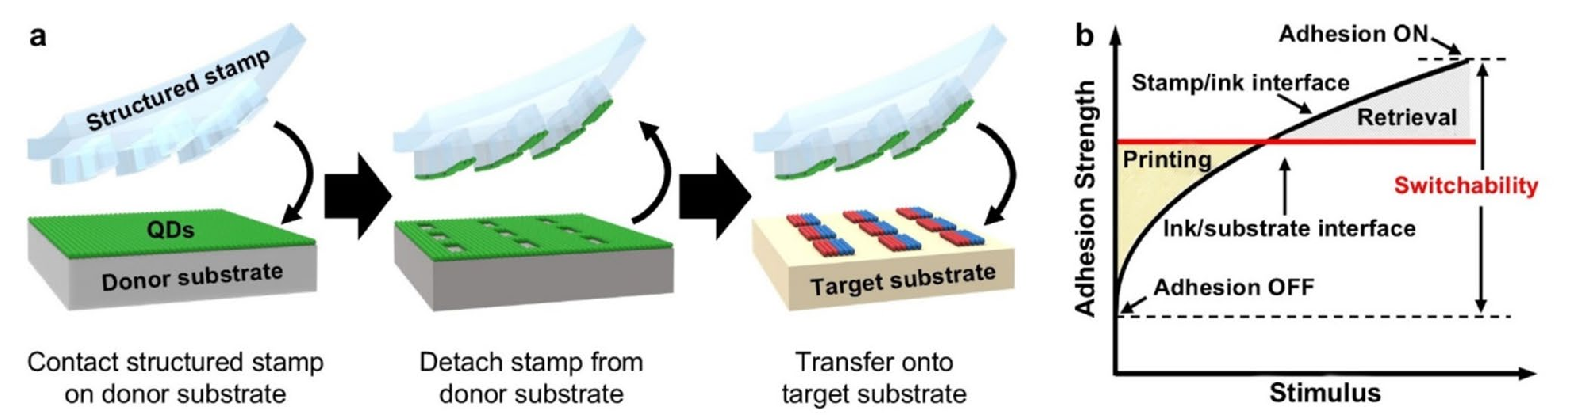
\includegraphics[width=0.85\textwidth]{p7.png}
\caption{微转印技术的工艺流程与粘附力调控原理\cite{kim2024recent}。左图：利用结构化印章实现量子点器件的图案化转移,展示了接触-拾取-转印三步骤过程,可实现RGB全彩像素的精确排列。右图：粘附力随外部刺激（温度/速度）的动态调控曲线。灰色区域（高刺激）对应拾取阶段，黑线高于红线，器件随印章移动；黄色区域（低刺激）对应转印阶段，黑线低于红线，器件释放到目标基底。这一原理确保了纳米级QLED器件在转移过程中不发生破损}
\label{fig:transfer_printing}
\end{figure}

\subsection{可呼吸的液态金属互连系统}

为了解决传统铜导线在运动出汗时阻挡湿气蒸发且易疲劳断裂的问题,本设计引入了\textbf{"液态金属纤维垫"}作为电路连接线\cite{ma2021permeable}。

\textbf{材料构成:} 采用Ma et al. (2021)开发的液态金属(EGaIn)涂层静电纺丝纤维垫(Liquid Metal Fiber Mat)。

\textbf{结构特性:}

\begin{itemize}
    \item \textbf{高透气性:} 不同于传统的实心导线,这种纤维垫具有多孔网状结构,透气率极高,允许汗液蒸汽自由穿透电路区域,防止因汗水积聚导致的短路或皮肤过敏。
    
    \item \textbf{超弹性导电:} 由于液态金属具有流体特性,该互连线在承受$>1800\%$的拉伸应变时,电阻变化率仅为微小值($\Delta R/R_0 < 1$),完美适配夜跑时的剧烈肢体摆动。
\end{itemize}

\begin{figure}[H]
\centering
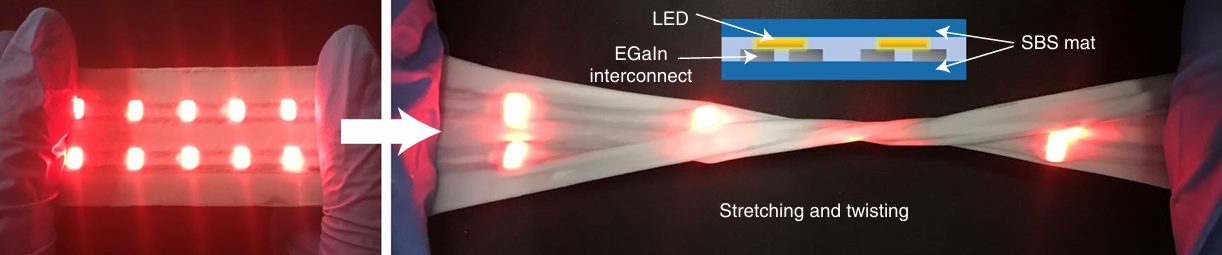
\includegraphics[width=0.9\textwidth]{p6.png}
\caption{液态金属纤维垫在拉伸和扭曲状态下的发光演示。左侧展示了贴附在手臂上的柔性LED阵列,右侧显示了器件在极端拉伸变形下仍能保持稳定发光,证明了液态金属互连系统的超高机械可靠性\cite{ma2021permeable}}
\label{fig:liquid_metal_demo}
\end{figure}

\subsection{系统封装与耐洗涤设计}

\textbf{封装材料:} 采用Parylene C(聚对二甲苯)进行真空气相沉积(CVD)。

\textbf{工艺优势:} Parylene C能在室温下形成致密的保形涂层(Conformal Coating),无针孔、厚度均匀($\sim$2$\,\mu$m)。

\textbf{耐洗涤性能:} 依据Fan et al. (2020)的测试标准,经过Parylene C封装的电子织物在经历40次以上的标准机洗循环(AATCC Test Method 135)后,功能层仍未发生剥离或电性能衰退,满足智能服装的日常维护需求\cite{fan2020machine}。

\begin{figure}[H]
\centering
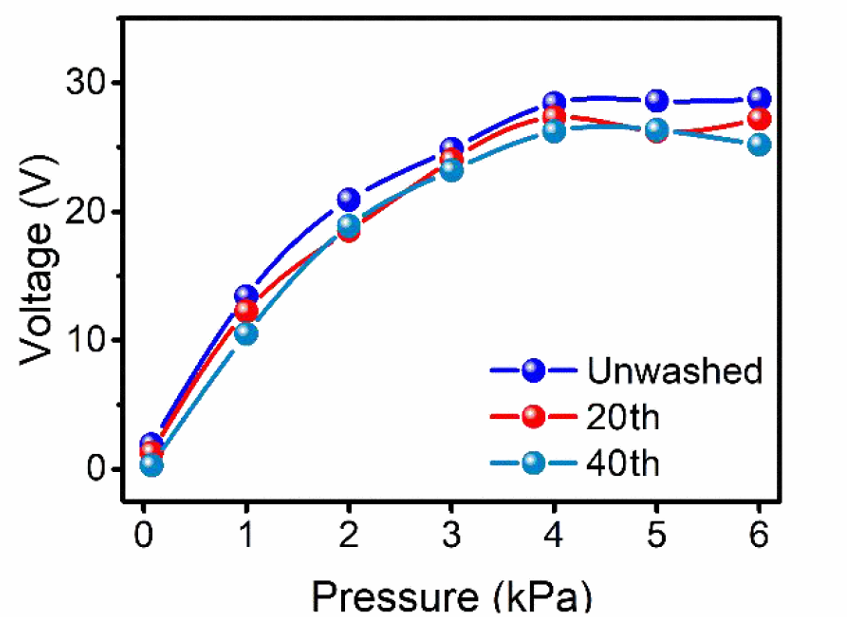
\includegraphics[width=0.75\textwidth]{p10.png}
\caption{电子织物传感器在多次洗涤后的性能稳定性测试\cite{fan2020machine}。图中展示了传感器在"Unwashed"（未洗涤）、"20th"（洗涤20次）和"40th"（洗涤40次）后的输出电压与压力关系曲线对比。三条曲线（深蓝、红、浅蓝）几乎完全重合，直接证明了在经历40次标准机洗循环后，器件的灵敏度和电学性能几乎没有衰减，验证了Parylene C封装技术的有效性。}
\label{fig:washability_test}
\end{figure}

\clearpage
\section{社会与环境方面的考虑}

\subsection{产业污染特征与环境风险分析}

在"流光守护"夜跑服的全生命周期中,必须正视不同制造阶段的潜在环境风险,以便采取针对性的阻断措施。

\subsubsection{量子点材料制造(QD Synthesis)}

\begin{itemize}
    \item \textbf{重金属毒性:} 当前高性能QLED仍主要依赖CdSe(硒化镉)。镉(Cd)属于I类致癌物,若在生产或废弃处理不当,会造成严重的土壤和水体重金属污染。
    
    \item \textbf{前驱体风险:} 合成过程涉及磷化氢(PH$_3$)等剧毒或易燃前驱体,对车间安全管控要求极高。
\end{itemize}

\subsubsection{器件制造(Device Fabrication)}

\begin{itemize}
    \item \textbf{溶剂污染:} 传统的旋涂工艺常使用氯苯(Chlorobenzene)或甲苯等芳香烃类有机溶剂。这些溶剂具有挥发性有机化合物(VOCs)排放风险,对人体神经系统有害。
    
    \item \textbf{能耗问题:} 高温退火和真空沉积工艺是主要的碳排放源。
\end{itemize}

\subsubsection{纺织品集成(Textile Integration)}

\textbf{微塑料排放:} 涤纶/氨纶面料在加工和洗涤过程中会释放微纤维(Microfibers),是水体微塑料污染的主要来源。

\subsection{绿色制造与清洁材料选择}

为降低上述风险,本设计提出以下"绿色升级"路线图:

\subsubsection{核心材料无毒化：从CdSe向InP过渡}

\textbf{短期方案:} 采用"核-壳-壳"致密封装技术(Core-Shell-Shell)。利用厚壳层ZnS将内部的CdSe完全包裹,防止镉离子泄漏,符合欧盟RoHS豁免标准。

\textbf{长期愿景:} 逐步替代为InP(磷化铟)无镉量子点。

\textbf{技术支撑:} 引用X Liu et al. (2025)的最新研究,通过优化ZnSe中间壳层的电子注入势垒,无镉InP QLED的外量子效率(EQE)已突破20\%,性能逼近含镉器件,为环保型夜跑服提供了技术可行性\cite{won2024green}。

\begin{figure}[H]
\centering
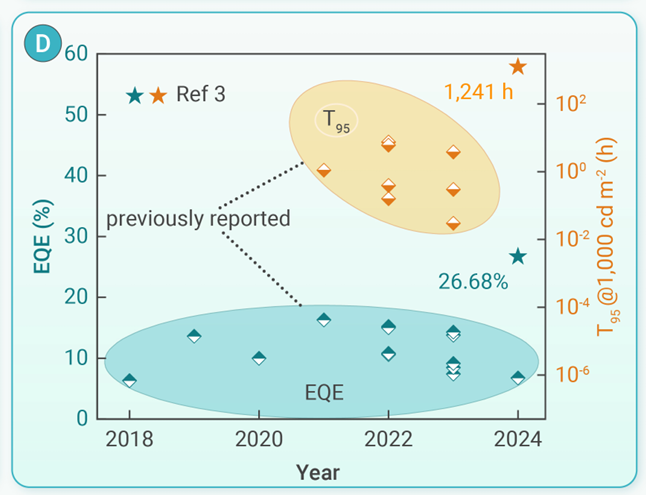
\includegraphics[width=0.8\textwidth]{p8.png}
\caption{InP QLED的EQE性能突破。图中的图表显示了EQE随年份的变化，其中标有一个显著的红星点"26.68\%"，展示了无镉量子点技术的性能里程碑。}
\label{fig:inp_qled_eqe}
\end{figure}

\subsubsection{绿色溶剂工艺(Green Solvent Processing)}

\textbf{溶剂优化策略:} 在器件制造中,需平衡环保性与工艺可行性:

\begin{itemize}
    \item \textbf{含TFB的三元发光层:} 由于TFB是非极性共轭聚合物,只能溶解于芳香烃溶剂(如氯苯、甲苯)。但可采用\textbf{低毒性替代品}如\textbf{邻二甲苯(o-Xylene)}或\textbf{均三甲苯(Mesitylene)},其毒性显著低于氯苯,且不在RoHS限制清单内\cite{kim2022green}。
    
    \item \textbf{ZnO电子传输层:} 使用水/乙醇混合溶剂,完全避免有机溶剂。
    
    \item \textbf{PEDOT:PSS空穴注入层:} 采用水基配方,无需有机溶剂。
\end{itemize}

\textbf{依据:} 研究表明,通过Hansen溶解度参数(HSP)筛选,邻二甲苯与氯苯的溶解性能相当($\delta \approx 18$ MPa$^{1/2}$),但其挥发性有机化合物(VOC)排放和职业暴露限值(OEL)均优于氯苯,是工业化生产的现实选择\cite{kim2022green}。

\subsubsection{低损耗转印技术(Loss-less Transfer)}

\textbf{减废效益:} 第五部分采用的"转印技术"具有显著的环保优势。它将复杂的化学处理(旋涂、蚀刻)限制在可回收的玻璃基底上进行,避免了化学试剂直接污染大面积的织物,从而减少了90\%以上的受污染纺织废料。

\subsection{废弃物处理与循环经济}

针对电子垃圾(E-waste)难以回收的痛点,本设计采用"模块化解体"策略:

\subsubsection{液态金属的回收再利用}

\textbf{回收原理:} 我们选用的EGaIn液态金属互连线具有独特的"可逆性"。在产品报废时,只需将织物浸泡在特定的碱性溶液中,液态金属即可与聚合物基质分离并汇聚成液滴回收,回收率可达94\%以上。

\textbf{技术支撑:} C Kim et al. (2025)在Small Science发表的研究证明,液态金属复合材料可以通过简单的化学过程实现闭环回收,重新用于制造新的电路,大幅降低了稀有金属(镓、铟)的资源消耗\cite{park2025recyclable}。

\begin{figure}[H]
\centering
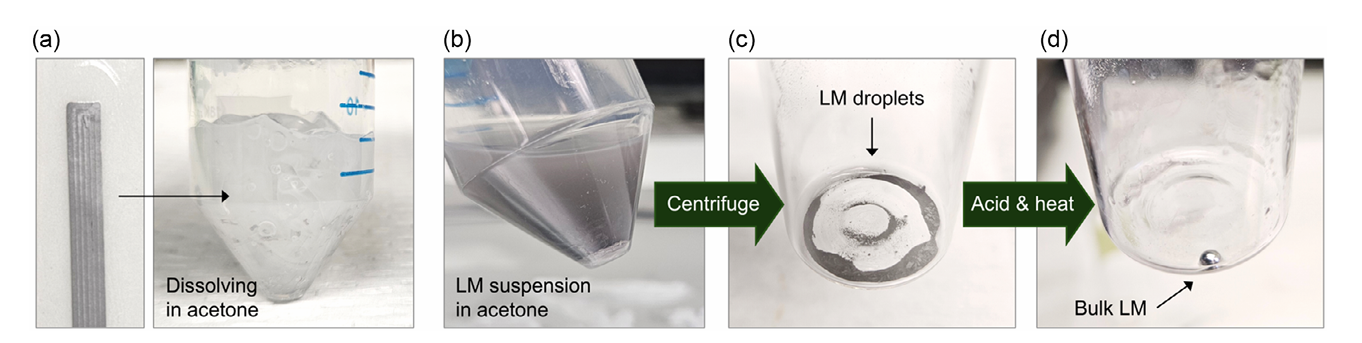
\includegraphics[width=1\textwidth]{p9.png}
\caption{液态金属完整回收流程示意图\cite{park2025recyclable}。(a) 溶解步骤：将印有液态金属复合材料的TPU基底浸泡在丙酮中，利用共聚物PASTA可溶于丙酮的特性，实现电子墨水层与织物/基底的分离。(b, c) 分离步骤：离心分离后，聚合物溶解在丙酮中，而液态金属（EGaIn）液滴因表面氧化物包裹沉淀到底部并保持分散状态。(d) 重组/回收步骤：加入乙酸并加热后，乙酸去除液滴表面的氧化层（生成乙酸镓），使得微小液滴重新融合成一整块大的液态金属球，实现材料的物理回收。}
\label{fig:liquid_metal_recycling}
\end{figure}

\subsubsection{织物与电子层分离}

利用TPU界面层的热塑性,通过加热至$150^{\circ}$C,可将QLED电子薄膜从织物上完整剥离。剥离后的织物可进入传统的衣物回收流程,而电子薄膜则送往专门的危废处理厂提取贵金属(银)。

\clearpage
\begin{thebibliography}{9}

\bibitem{kim2024intrinsically}
Kim, D.-H., et al.
\textit{Intrinsically stretchable quantum dot light-emitting diodes}.
Nature Electronics, 2024, 7: 1--10.

\bibitem{choi2023highly}
GW Baek, et al.
\textit{Highly Bright and Efficient Flexible Quantum Dot Light-Emitting Diodes on Metal-Coated PEN Substrate}.
Journal of Flexible and Printed Electronics, 2023, 2: 1--12.

\bibitem{chen2022high}
H Yu, et al.
\textit{High-Efficiency, Large-Area, Flexible Top-Emitting Quantum-Dot Light-Emitting Diode}.
ACS Photonics, 2022, 9(11): 3567--3575.

\bibitem{haghighi2023investigation}
S Mokarian Zanjani, et al.
\textit{An investigation on the cyclic temperature-dependent performance behaviors of ultrabright air-stable QLEDs}.
Scientific Reports, 2023, 13: 14568.

\bibitem{lee2023truly}
Lee, S., Choi, H.W., et al.
\textit{Truly form-factor-free industrially scalable system integration for electronic textile architectures with multifunctional fiber devices}.
Science Advances, 2023

\bibitem{bang2021technology}
Bang, S.Y., Suh, Y.-H., Fan, X.-B., Shin, D.-W., Lee, S., Choi, H.W., Lee, T.H., Yang, J., Zhan, S., Harden-Chaters, W., et al.
\textit{Technology progress on quantum dot light-emitting diodes for next-generation displays}.
Nanoscale Horizons, 2021, 6(2): 68--77.

\bibitem{kim2024recent}
Kim, Y., Yang, J., \& Choi, M.K.
\textit{Recent Advances in Transfer Printing of Colloidal Quantum Dots for High-Resolution Full Color Displays}.
Korean Journal of Chemical Engineering, 2024.
DOI: 10.1007/s11814-024-00301-3.

\bibitem{ma2021permeable}
Ma, Z., et al.
\textit{Permeable superelastic liquid-metal fibre mat enables biocompatible and monolithic stretchable electronics}.
Nature Materials, 2021.
DOI: 10.1038/s41563-020-00902-3.

\bibitem{fan2020machine}
Fan, W., et al.
\textit{Machine-knitted washable sensor array textile for precise epidermal physiological signal monitoring}.
Science Advances, 2020.
DOI: 10.1126/sciadv.aay2840.

\bibitem{won2024green}
X Liu., et al.
\textit{Green InP-based quantum dot light-emitting diodes made efficient and stable}.
The Innovation Materials, 2025.

\bibitem{kim2022green}
HB Kim, ., et al.
\textit{Green Solvent Selection for All Solution-Processed Inverted Quantum Dot Light-Emitting Diodes}.
Advanced Functional Materials, 2024.

\bibitem{park2025recyclable}
C Kim., et al.
\textit{Recyclable Printed Liquid Metal Composite for Underwater Stretchable Electronics}.
Small Science, 2025.

\end{thebibliography}

\end{document}